\documentclass{article}

\usepackage[a4paper, top=35mm, bottom=40mm, right=30mm, left=30mm]{geometry}
\usepackage[ngerman]{babel}
\usepackage[utf8x]{inputenc}
\usepackage[T1]{fontenc}
\usepackage{mathtools}
\usepackage{textcomp}
\usepackage{graphicx}
\usepackage{tabularx}
\usepackage{amssymb}
\usepackage{pifont}
\newcommand{\cmark}{\ding{51}}%
\newcommand{\xmark}{\ding{55}}%
\setlength{\parindent}{0pt}
\linespread{1.6}

\title{Crawling von Datenschutzhistorien}
\author{Alexander Prull, Jörn-Henning Daug, Simon Kaleschke}
\date{Februar 2017}

\begin{document}
	
	\maketitle
	
	\section{Projektbeschreibung}
	
	\section{Lösungsansatz}
	
	\section{Softwarearchitektur}
	Die Software ist in drei Teile aufgeteilt: Frontend, Backend, und Extraktion.
	
	\subsection{Frontend}
	\subsection{Backend}
	\subsection{Extraktion}
	Die Ruby-Struktur zur Extraktion der Datenschutzhistorien funktioniert folgendermaßen:
	
	Vom Backend aus wird \textit{crawl.rb} aufgerufen. Dieses Skript beinhaltet alle Einstellungen zur Extraktion von jeder Webseite. Es sendet diese Einstellungen an \textit{PrivacyExtractor.rb}, das die Extraktion dann vollzieht. Hierfür bezieht es Links zu älteren Versionen entweder vom Archiv der Webseite selbst, oder mit \textit{ArchiveExtractor.rb} von dem Internetarchiv \textit{archive.org}. Der Inhalt jeder Seite wird extrahiert, auf die notwenigen Elemente zugeschnitten und formatiert. Zuletzt werden mit \textit{PrivacyDiffer.rb} die extrahierten Texte auf Unterschiede untersucht und gegebenenfalls in einer Datenbank abgespeichert. Die fertige Datenbank kann vom Frontend weiterverarbeitet werden.
	
	Weitere Informationen sind auf der Abbildung \ref{fig:uml-ex} auf Seite \pageref{fig:uml-ex} zu finden.
	
	\section{Bedienungsanleitung}
	\subsection{Vorbereitung}
	Damit die Software reibungslos läuft, werden folgende vorinstallierte Pakete erwartet:
	
	Für das Frontend:
	\begin{itemize}
		\item Bower.
		\item ...
	\end{itemize}

	Für das Backend:
	\begin{itemize}
		\item Java.
		\item SQLite3.
		\item Maven.
		\item ...
	\end{itemize}

	Für die Extraktion:
	\begin{itemize}
		\item Ruby 2.3.1 oder höher.
		\item Die Ruby-Gems \textit{date, open-uri, open\_uri\_redirections, nokogiri, rubygems, sqlite3, json, differ}.
	\end{itemize}

	Tragen sie außerdem in der Datei \textit{config.ppp} den von Ihnen gewünschten Pfad für die Ergebnisdatenbank ein. (Standard ist \textit{$\sim$/html/policies.db}) 
	\subsection{Server einrichten}
	\subsection{Serverstart und allgemeiner Programmablauf}
	\subsection{Webseite einzeln crawlen}
	Normalweise wird der Aufruf zur Extraktion vom Backend aus gestartet. Wollen Sie jedoch eine einzelne Webseite crawlen, gehen sie folgendermaßen vor:
	\begin{enumerate}
		\item Sichern Sie, dass die Webseite und zugehörige Optionen im Quellcode vermerkt ist. (Siehe dazu Abschnitt \ref{sec:add-site})
		\item Sind noch keine Informationen zu der Webseite vorhanden, oder wollen Sie alle Informationen von null an neu generieren lassen, wechseln sie in den Ordner \textit{script} und starten sie den Aufruf \texttt{ruby crawl.rb webseite fetch}. Wollen sie bspw. alle Informationen für Google neu generieren lassen, ersetzen sie im Aufruf \texttt{webseite} durch \texttt{google}.
		\item Wollen Sie nun überprüfen, ob eine neue Version verfügbar ist, starten Sie den Aufruf \texttt{ruby crawl.rb webseite update}.
	\end{enumerate}
	
	\subsection{Datenbankstruktur}
		Die SQLite-Datenbank hat folgende Spalten:
		
		\begin{tabularx}{\textwidth}{|r|X|}
			\hline
			\textbf{Spalte} & \textbf{Bedeutung} \\ \hline \hline
			ID & Primärschlüssel. \\ \hline
			SYSTEM\_DATE & Datum, an dem die Datenschutzhistorie in dem aktuellen Zustand war.\\ \hline
			DISPLAY\_DATE & Gleiches Datum in benutzerfreundlicher Schreibweise. \\ \hline
			LINK & Hyperlink, wo die extrahierte Historie zu finden ist.\\ \hline
			CONTENT & Der extrahierte Plaintext.\\ \hline
		\end{tabularx}
	
	
	\section{Ergebnisse} 
	\subsection{Allgemeines}
	[...]
	
	Eine Liste aller gecrawlten Webseiten ist auf Abbildung \ref{fig:crawl-tab} auf Seite \pageref{fig:crawl-tab} zu finden.
	\subsection{Die Website}
	
	\section{Einschränkungen}
	
	\section{Erweiterungsmöglichkeiten}
	\subsection{Daten weiterverarbeiten}
	Die gewonnenen Daten in der Datenbank können unabhängig von der Webseite vielseitig weiterverwendet werden. so wäre bspw. die Anbindung an weiter Anwendungsprogramme, zum Beispiel zur Bewertung der Datenqualität oder zur Suche nach Schlüsselwörtern, möglich.
	\subsection{Webseite hinzufügen}
	\label{sec:add-site}
	Wenn Sie eine Webseite zum Tool hinzufügen möchten, so brauchen Sie i.A. den Namen der Webseite und einen Hyperlink zur Webseite, auf der die Datenschutzerklärung zu finden ist. Wie weiter vorzugehen ist, wird im folgenden beschrieben:
	\subsubsection{Frontend}
	\subsubsection{Backend}
	[...]
	
	Fügen Sie außerdem in \textit{crawl.rb} den Namen der Webseite, den Link, den Namen der Tabelle, in der die Informationen gespeichert werden sollen, wie die HTML-Struktur zu modifizieren ist, etc. ein. Näheres wird mit Beispielen im Skript selbst erläutert.
	
	\newpage
	\section{Anhang}
	\begin{figure}[ht]
		\centering
		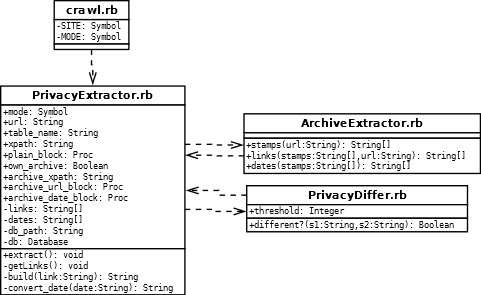
\includegraphics[width=0.75\textwidth]{extraction}
		\caption{Architektur Extraktion}
		\label{fig:uml-ex}
	\end{figure}
	\begin{figure}[ht]
		\centering
		\begin{tabularx}{\textwidth}{|r|c|c|c|X|}
			\hline
			\textbf{Firma} & \textbf{Eigenes Archiv} & \textbf{Versionen} & \textbf{Zeitspanne} & \textbf{Qualität} \\ \hline \hline
			Alternate & \xmark & 7 & 08/2014 - 07/2016 &  0.9 \\ \hline
			Amorelie & \xmark & 11 & 01/2013 - 10/2016 &  0.7 \\ \hline
			Apple & \xmark & 12 & 09/2014 - 09/2016 &  1.0 \\ \hline
			Burgerking & \xmark & 2 & 02/2015 - 12/2016 &  0.7 \\ \hline
			Edeka & \xmark & 4 & 11/2014 - 10/2016 &  0.7 \\ \hline
			Google & \cmark & 22 & 06/1999 - 01/2017 &  0.8 \\ \hline
			Microsoft & \xmark & 7 & 02/2016 - 01/2017 &  0.9 \\ \hline
			Payback & \xmark & 10 & 09/2011 - 10/2016 &  0.9 \\ \hline
			Paypal & \xmark & 2 & 04/2014 - 11/2016 &  0.9 \\ \hline
			RocketbeansTV & \xmark & 4 & 10/2014 - 09/2016 &  1.0 \\ \hline
			Steam & \xmark & 3 & 09/2012 - 11/2016 &  0.8 \\ \hline
			Subway & \xmark & 3 & 05/2016 - 10/2016 &  0.9 \\ \hline
			Süddeutsche & \xmark & 1 & 04/2015 - 04/2015 &  0.2 \\ \hline
			Trivago & \xmark & 1 & 04/2016 - 04/2016 &  0.7 \\ \hline
			Twitter & \cmark & 10 & 05/2007 - 01/2016 &  0.8 \\ \hline
			Uni Leipzig & \xmark & 1 & 06/2013 - 06/2013 &  0.5 \\ \hline
			Vine & \xmark & 5 & 03/2013 - 01/2017 &  1.0 \\ \hline
			WhatsApp & \cmark & 2 & 07/2012 - 01/2017 &  0.9 \\ \hline
			Wikimedia & \cmark & 4 & 06/2006 - 06/2014 &  1.0 \\ \hline
			Zalando & \xmark & 3 & 09/2010 - 11/2012 &  0.9 \\ \hline
		\end{tabularx}
		\caption{Übersicht gecrawlte Webseiten}
		\label{fig:crawl-tab}
	\end{figure}
	
\end{document}